\section{Methods}

\subsection{Transformers}

In the works of NLP, the use of pre-entrained language models hace become a useful block to get a better result on every task. One of the most competitive neural sequence transduction models have an encoder-decoder structure\cite{Bahdanau_2014,Cho_2014}. Here, the encoder maps an input sequence of symbol representations $(x_1 , \dots, x_n)$ to a sequence of continuous representations $z = (z_1 , \dots, z_n )$. Given z, the decoder then generates an output sequence $(y_1 , \dots, y_m )$ of symbols one element at a time. At each step the model is auto-regressive\cite{Graves_2013}, consuming the previously generated symbols as additional input when generating the next. The Transformer follows this overall architecture using stacked self-attention and point-wise, fully connected layers for both the encoder and decoder (figure \ref{fig:transformer}). The encoder is composed of a stack of N = 6 identical layers. Each layer has two sub-layers. The first is a multi-head self-attention mechanism, and the second is a simple, position wise fully connected feed-forward network.

\begin{figure}[H]
    \centering
    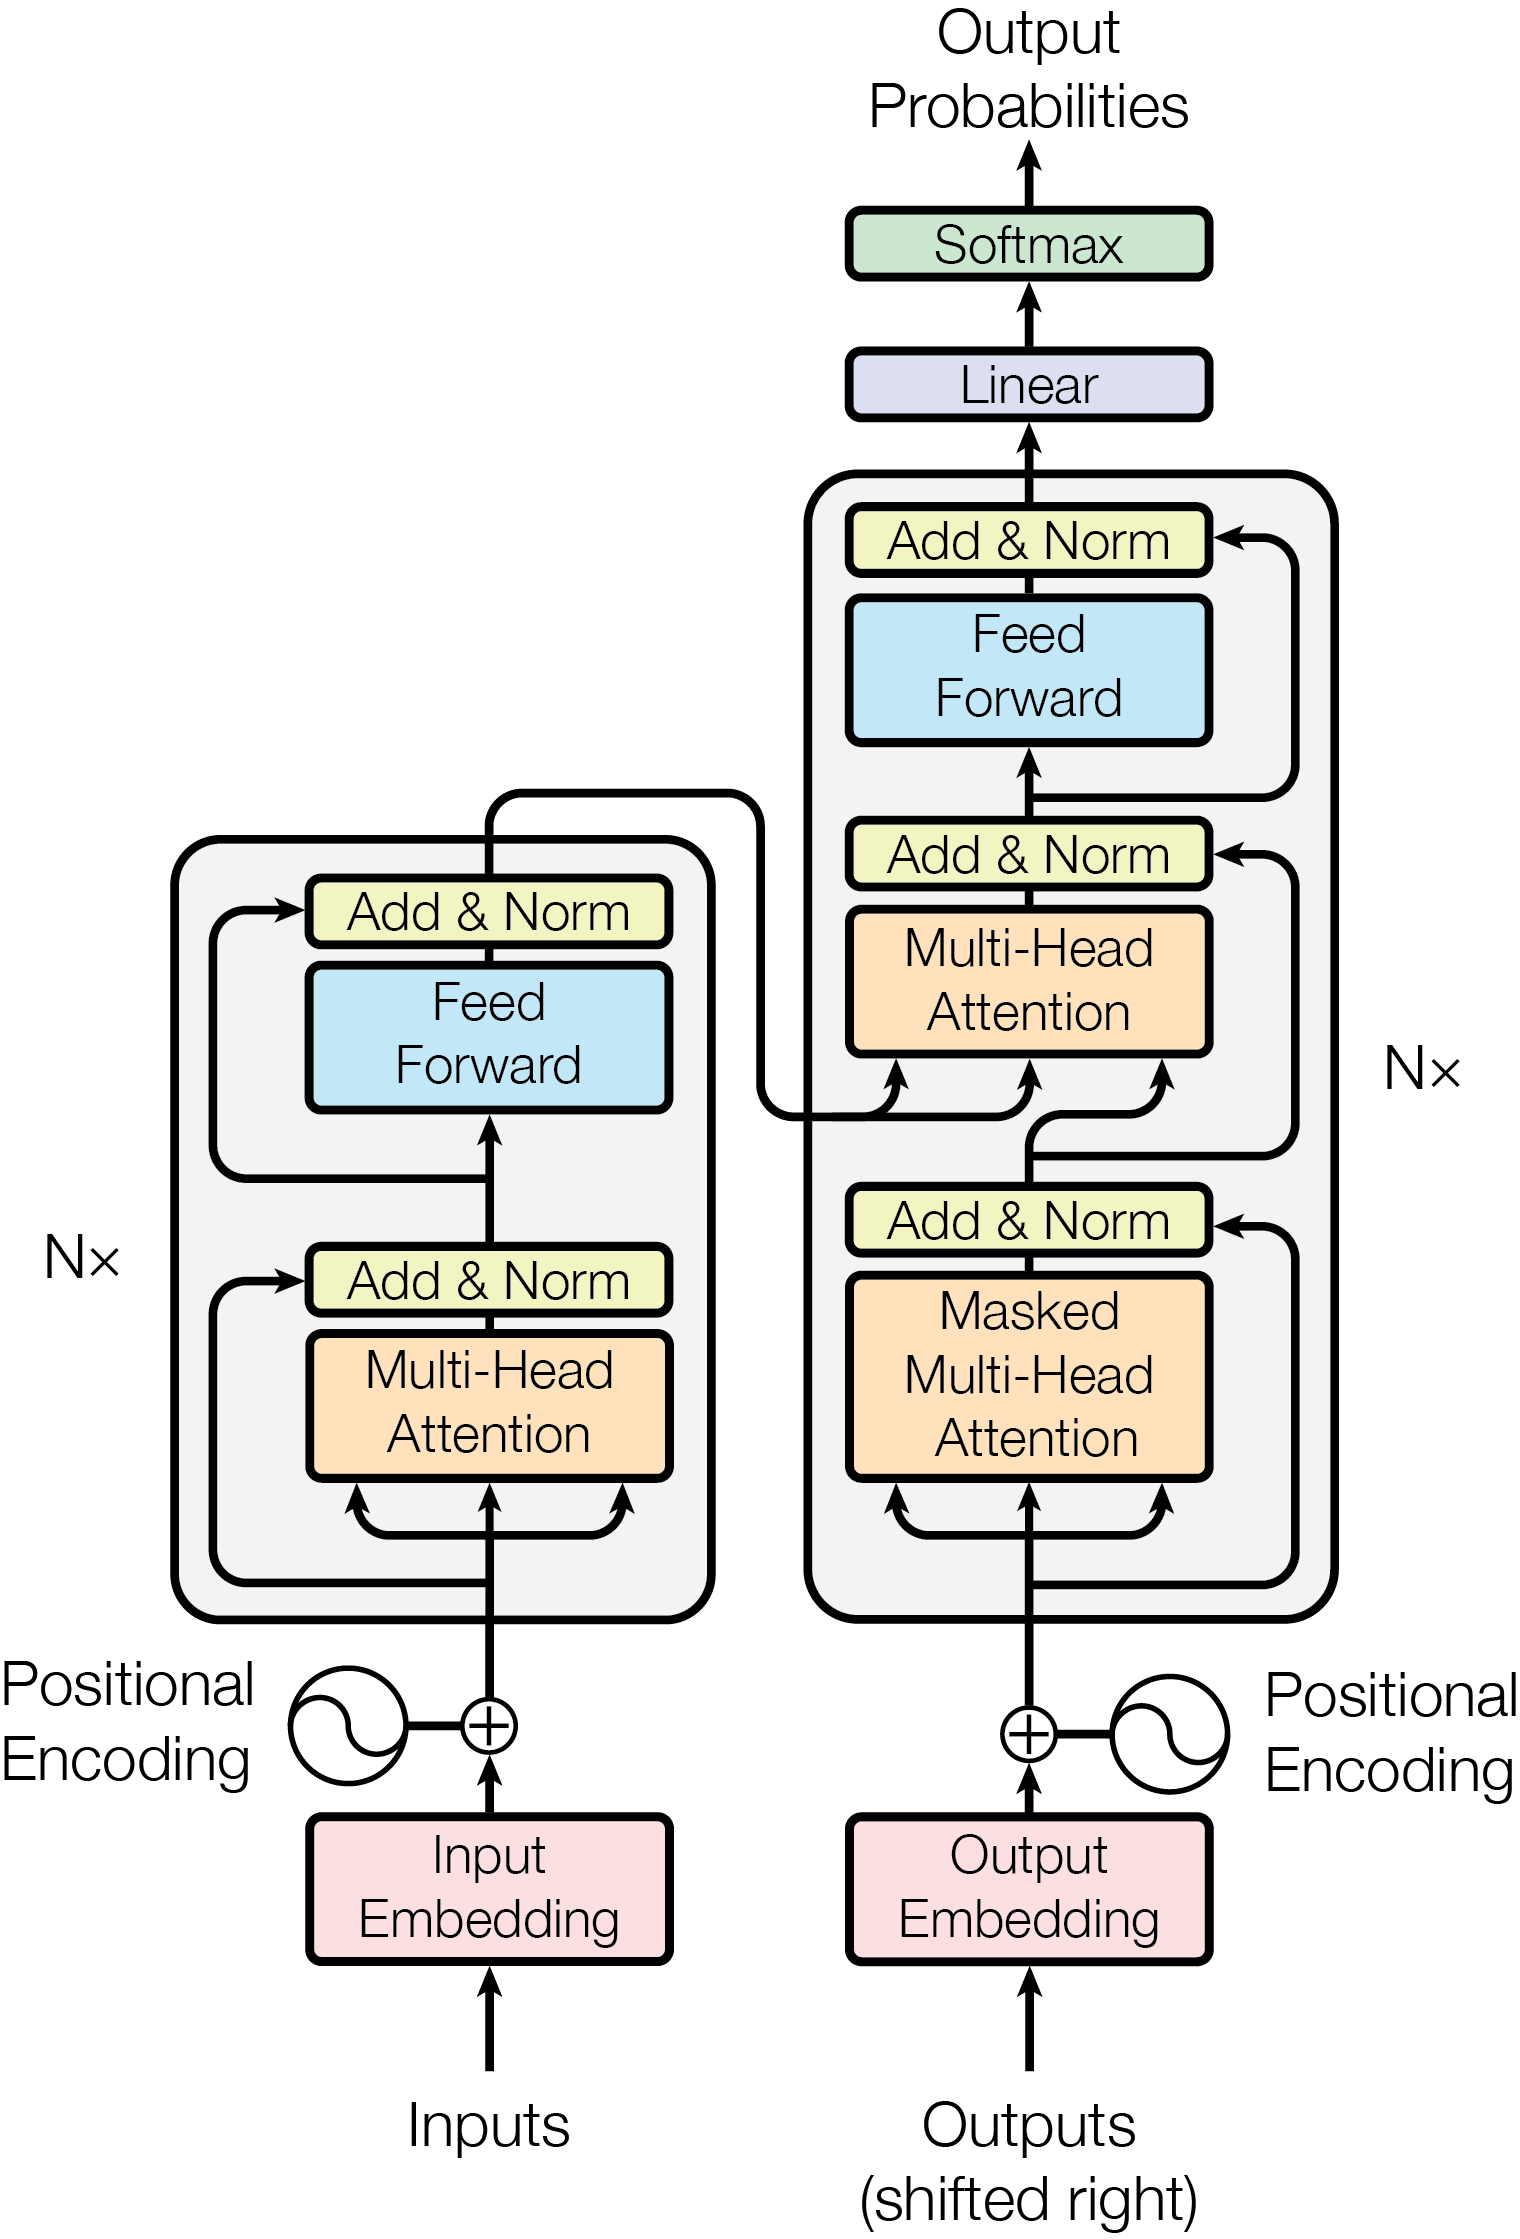
\includegraphics[width=6cm]{Graphics/transformer.png}
    \caption{Transformer model representation\cite{Vaswani_2017}.}
    \label{fig:transformer}
\end{figure}

\subsection{Bert}

\subsection{Robertuito}

\subsection{MEX-A3T}

\begin{table}[H]
    \centering
    \changefontsizes{9pt}
    \begin{tabular}{lrrrrrr} \hline
        \\
        \textbf{Team Name}          & \textbf{F1 offensive} & \textbf{F1 non-offensive} & \textbf{F1 macro} & \textbf{Precision} & \textbf{Recall} & \textbf{Accuracy} \\ \hline
        \\[-0.1cm]
        \textbf{CIMAT-1}            & 0.7998                & 0.9195                    & 0.8596            & 0.8605             & 0.8588          & 0.8851            \\[0.05cm]
        \textbf{CIMAT-2}            & 0.7971                & 0.9205                    & 0.8588            & 0.8641             & 0.8540          & 0.8858            \\[0.05cm]
        \textbf{UPB-2}              & 0.7969                & 0.9107                    & 0.8538            & 0.8440             & 0.8668          & 0.8759            \\[0.05cm]
        \textbf{UACh-2}             & 0.7720                & 0.9042                    & 0.8381            & 0.8332             & 0.8437          & 0.8651            \\[0.05cm]
        \textbf{INGEOTEC}           & 0.7468                & 0.8933                    & 0.8200            & 0.8150             & 0.8258          & 0.8498            \\[0.05cm]
        \textbf{Idiap-UAM-1}        & 0.7255                & 0.8886                    & 0.8071            & 0.8067             & 0.8075          & 0.8416            \\[0.05cm]
        \textbf{Baseline (Bi-GRU)}  & 0.7124                & 0.8841                    & 0.7983            & 0.7988             & 0.7978          & 0.8348            \\[0.05cm]
        \textbf{Idiap-UAM-2}        & 0.7066                & 0.8953                    & 0.8010            & 0.8234             & 0.7860          & 0.8457            \\[0.05cm]
        \textbf{UACh-1}             & 0.7062                & 0.8861                    & 0.7961            & 0.8021             & 0.7909          & 0.8358            \\[0.05cm]
        \textbf{DeepMath-1}         & 0.7001                & 0.8544                    & 0.7773            & 0.7662             & 0.8120          & 0.8040            \\[0.05cm]
        \textbf{DeepMath-2}         & 0.6957                & 0.8537                    & 0.7747            & 0.7639             & 0.7971          & 0.8024            \\[0.05cm]
        \textbf{Baseline (BoW-SVM)} & 0.6760                & 0.8780                    & 0.7770            & -                  & -               & 0.8228            \\[0.05cm]
        \textbf{UMUTeam-2}          & 0.6727                & 0.8706                    & 0.7716            & 0.7744             & 0.7691          & 0.8145            \\[0.05cm]
        \textbf{Intensos-1}         & 0.6619                & 0.8752                    & 0.7686            & 0.7820             & 0.7588          & 0.8177            \\[0.05cm]
        \textbf{UMUTeam-3}          & 0.6516                & 0.8771                    & 0.7644            & 0.7868             & 0.7503          & 0.8183            \\[0.05cm]
        \textbf{Ugalileo-2}         & 0.6388                & 0.8208                    & 0.7298            & 0.7213             & 0.7531          & 0.7604            \\[0.05cm]
        \textbf{Ugalileo-1}         & 0.6387                & 0.8430                    & 0.7408            & 0.7350             & 0.7486          & 0.7811            \\[0.05cm]
        \textbf{ITCG-SD}            & 0.6080                & 0.8820                    & 0.7450            & 0.8133             & 0.7203          & 0.8186            \\[0.05cm]
        \textbf{UMUTeam-1}          & 0.5892                & 0.8430                    & 0.7161            & 0.7223             & 0.7112          & 0.7728            \\[0.05cm]
        \textbf{UPB-1}              & 0.3437                & 0.8463                    & 0.5950            & 0.7333             & 0.5947          & 0.7509            \\[0.05cm]
        \textbf{Intensos-2}         & 0.2515                & 0.7664                    & 0.5090            & 0.5189             & 0.5141          & 0.6440            \\[0.05cm] \hline
    \end{tabular}
    \normalsize
    \caption{Results for aggressiveness identification in the IberLEF 2020.}
    \label{table:agIberLEF_2020}
\end{table}